\renewcommand{\thesection}{\arabic{section}}\renewcommand{\theHsection}{chapter.\arabic{section}}\setcounter{section}{2}\section{运动方程的积分}
\noindent\begin{minipage}{\textwidth}\ProblemHeading{例题}{3.1（改写）}
质量为 $m$ 的质点沿 $x$ 轴运动。图中实线为势能 $U(x)$，水平虚线为给定的总能量 $E$，$x$ 向右增大。指出质点可达的区间及各区间的有限边界，并判断各允许区间中的运动是有界还是无界。
\begin{center}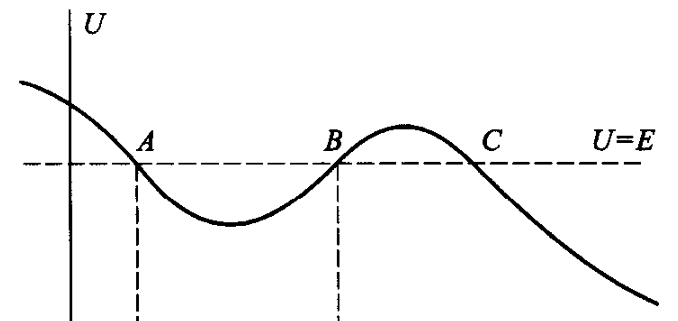
\includegraphics[width=0.43\linewidth]{figures/fig_3_1_1.png}\end{center}
\end{minipage}\par\vfill
\noindent\begin{minipage}{\textwidth}\ProblemHeading{习题}{3.2}
质量为 $m$、摆长为 $l$ 的平面单摆在重力加速度为 $g$ 的均匀重力场中振动。求振动周期随最大摆角 $\varphi_0$ 的变化关系。
\end{minipage}\par\vfill
\newpage
\noindent\begin{minipage}{\textwidth}\ProblemHeading{习题}{3.3}
质量为 $m$ 的质点沿 $x$ 轴运动。对于下列势能 $U(x)$，求有界振动的周期 $T$ 随总能量 $E$ 的变化关系。
\SubQ{1}{$U(x)=A|x|^n$。}
\SubQ{2}{$U(x)=-U_0/\cosh^2(\alpha x)$，其中 $-U_0<E<0$。}
\SubQ{3}{$U(x)=U_0\tan^2(\alpha x)$，取含 $x=0$ 的势阱。}
\end{minipage}\par\vfill
\noindent\begin{minipage}{\textwidth}\ProblemHeading{习题}{3.4}
一个封闭质点系由一个质量为 $M$ 的质点和 $n$ 个质量均为 $m$ 的质点组成，各质点间的势能只依赖于它们之间的距离。消去质心运动，把原系统的运动化为 $n$ 体问题。
\end{minipage}\par\vfill
\newpage
\noindent\begin{minipage}{\textwidth}\ProblemHeading{例题}{3.5（改写）}
一质点以非零动量矩在有心力场中作有界运动，径向运动有两个简单转折点 $r_{\min}$ 与 $r_{\max}$。设质点从一个最远点出发，经过最近点，到达下一个最远点，径矢转过 $\Delta\varphi$。
\SubQ{1}{说明最近点两侧相邻的两段轨道为何关于经过该点的径向直线对称。}
\SubQ{2}{用 $\Delta\varphi$ 表示轨道闭合的条件。}
\end{minipage}\par\vfill
\noindent\begin{minipage}{\textwidth}\ProblemHeading{习题}{3.6}
质量为 $m$ 的质点在均匀重力场中受约束沿半径为 $l$ 的球面运动，构成球面摆。试积分球面摆的运动方程。
\end{minipage}\par\vfill
\newpage
\noindent\begin{minipage}{\textwidth}\ProblemHeading{习题}{3.7}
一质点在均匀重力场中沿一竖直圆锥的锥面运动。圆锥的顶角为 $2\alpha$，顶点朝下。试积分该质点的运动方程。
\end{minipage}\par\vfill
\noindent\begin{minipage}{\textwidth}\ProblemHeading{习题}{3.8}
如图，一平面摆的摆球质量为 $m_2$，摆长为 $l$，质量为 $m_1$ 的悬挂点可沿水平直线运动。设重力加速度为 $g$，试积分该摆的运动方程。
\begin{center}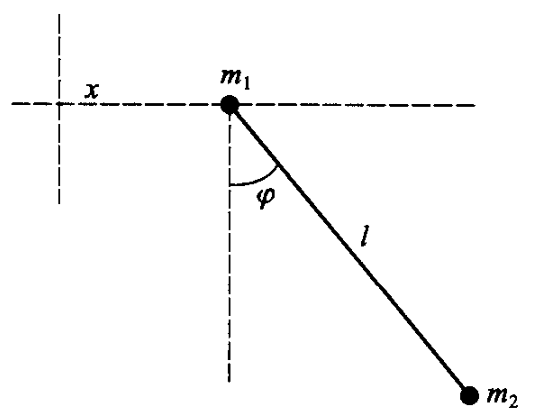
\includegraphics[width=0.28\linewidth]{figures/fig_3_8_1.png}\end{center}
\end{minipage}\par\vfill
\newpage
\noindent\begin{minipage}{\textwidth}\ProblemHeading{例题}{3.9（改写）}
质量为 $m$ 的质点在势能 $U(r)=-\alpha/r$（$\alpha>0$）的有心力场中运动，动量矩大小为 $M>0$，总能量为 $E$。
\SubQ{1}{求有效势能的极小值及取到它的半径。}
\SubQ{2}{求轨道的极坐标方程，并分别判断 $E<0$ 与 $E>0$ 时轨道的形状。}
\SubQ{3}{当 $E<0$ 时，求椭圆轨道的半长轴、半短轴和运动周期。}
\end{minipage}\par\vfill
\noindent\begin{minipage}{\textwidth}\ProblemHeading{例题}{3.10（改写）}
质量为 $m$ 的质点在吸引场 $U(r)=-\alpha/r$（$\alpha>0$）中运动，动量矩大小为 $M>0$。在轨道平面内取力心为坐标原点，$x$ 轴正向指向近心点，质点通过该点时取 $t=0$。分别把位置 $(x,y)$ 和时间 $t$ 写成同一轨道参数的函数。
\SubQ{1}{质点沿非圆的椭圆轨道运动。}
\SubQ{2}{质点沿双曲线轨道运动。}
\end{minipage}\par\vfill
\newpage
\noindent\begin{minipage}{\textwidth}\ProblemHeading{例题}{3.11（改写）}
质量为 $m$ 的质点在势能 $U(r)=\alpha/r$（$\alpha>0$）的斥力场中运动，动量矩大小为 $M>0$，总能量为 $E$。说明为什么这种运动一定无界，求轨道的极坐标方程和近心距离。
\end{minipage}\par\vfill
\noindent\begin{minipage}{\textwidth}\ProblemHeading{例题}{3.12（改写）}
质量为 $m$ 的质点在有心力场 $U(r)=\alpha/r$ 中运动，$\alpha$ 的符号任意。记质点的径矢、速度和动量矩为 $\mathbf r$、$\mathbf v$ 和 $\mathbf M$。
\SubQ{1}{证明 $\mathbf A=\mathbf v\times\mathbf M+\alpha\mathbf r/r$ 沿轨道保持不变。}
\SubQ{2}{对有近心点且偏心率 $e>0$ 的非径向轨道，在近心点计算 $\mathbf A$，确定其大小和方向。}
\end{minipage}\par\vfill
\newpage
\noindent\begin{minipage}{\textwidth}\ProblemHeading{习题}{3.13}
质点在势能 $U(r)=-\alpha/r$（$\alpha>0$）的有心力场中沿抛物线运动，其总能量 $E=0$。求质点坐标与时间的关系。
\end{minipage}\par\vfill
\noindent\begin{minipage}{\textwidth}\ProblemHeading{习题}{3.14}
质点在势能 $U(r)=-\alpha/r^2$（$\alpha>0$）的有心力场中运动。试积分运动方程。
\end{minipage}\par\vfill
\newpage
\noindent\begin{minipage}{\textwidth}\ProblemHeading{习题}{3.15（校订）}
在吸引势能 $U(r)=-\alpha/r$（$\alpha>0$）上加一小量 $\delta U(r)$。考虑原本沿椭圆轨道运动的质点，求下列扰动导致的每一径向周期内近心点方位角的一阶改变量 $\delta\varphi$。
\SubQ{1}{$\delta U(r)=\beta/r^2$。}
\SubQ{2}{$\delta U(r)=\gamma/r^3$。}
\end{minipage}\par\vfill
